\vspace{10pt}

{\centering\subsection*{雷欣悦:春风吹,风筝飞}}

\addcontentsline{toc}{subsection}{雷欣悦:春风吹,风筝飞}

\renewcommand{\leftmark}{雷欣悦:春风吹,风筝飞}

\begin{figure}[htbp]

\centering

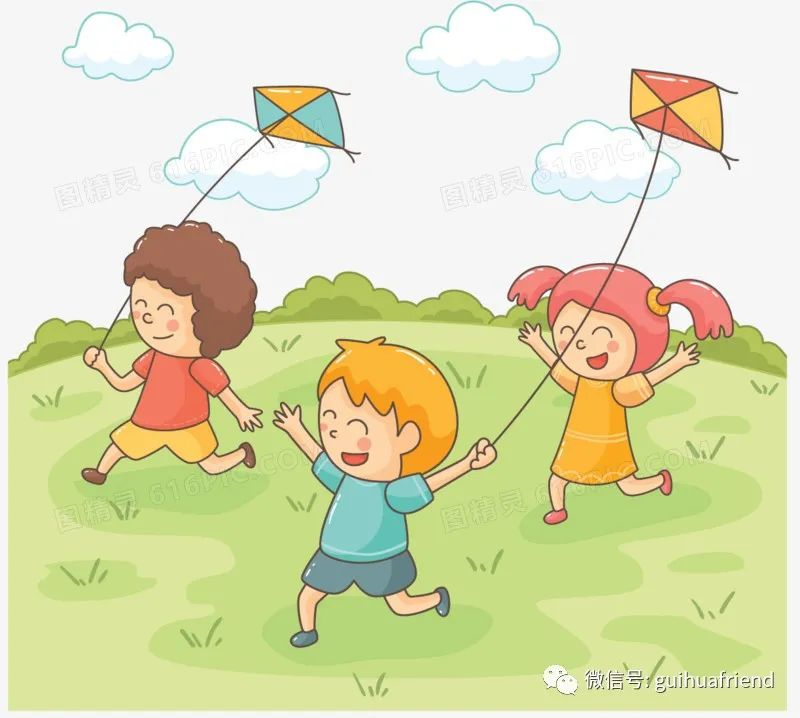
\includegraphics[width = .5\textwidth]{./ch/24.jpg}

\end{figure}





春天来了,桃花红了,杏花白了,风也暖和了,孩子们来到碧绿的草地上,放起了风筝。

我们来到公园,一进去就看到有三个小朋友,一个叫乐乐,另一个小男孩叫小军,还有一个小女孩叫小红。

乐乐拿着风筝线,小军把风筝高高举起,乐乐嘴里嘀咕着:我终于可以放美丽的风筝啰!天上的白云高高的挂在蓝天上,地面上的青草和鲜花五颜六色的。各种各样的风筝,在天空上飞翔。小红看见了乐乐高高飞起的风筝。也想尝试放风筝。

草长莺飞二月天,许许多多人都在草地上放风筝。这真的是一幅美好的画面,我好想用我珍贵的水彩笔把这美好的画面给画下来。我爱这春天美好的风景!





\vspace{10pt}



作者:三(1)班 雷欣悦



指导老师:谢婷



投稿:2021年5月13日



发表:2021年5月14日










                



\vspace{10pt}

\hline



